



\documentclass[10pt]{article}
\usepackage{threeparttable}
\usepackage{apacite}
\usepackage{graphicx}
\usepackage{multicol}
\usepackage{multirow}
\usepackage{caption}
\usepackage{extarrows}%为了输出长等号
\usepackage{subcaption}%为了插图
\usepackage[UTF8]{ctex}

\begin{document}


\begin{figure}[h!]
\begin{multicols}{2}   
    \begin{minipage}[h]{0.5\textwidth} 
        \centering   
        % 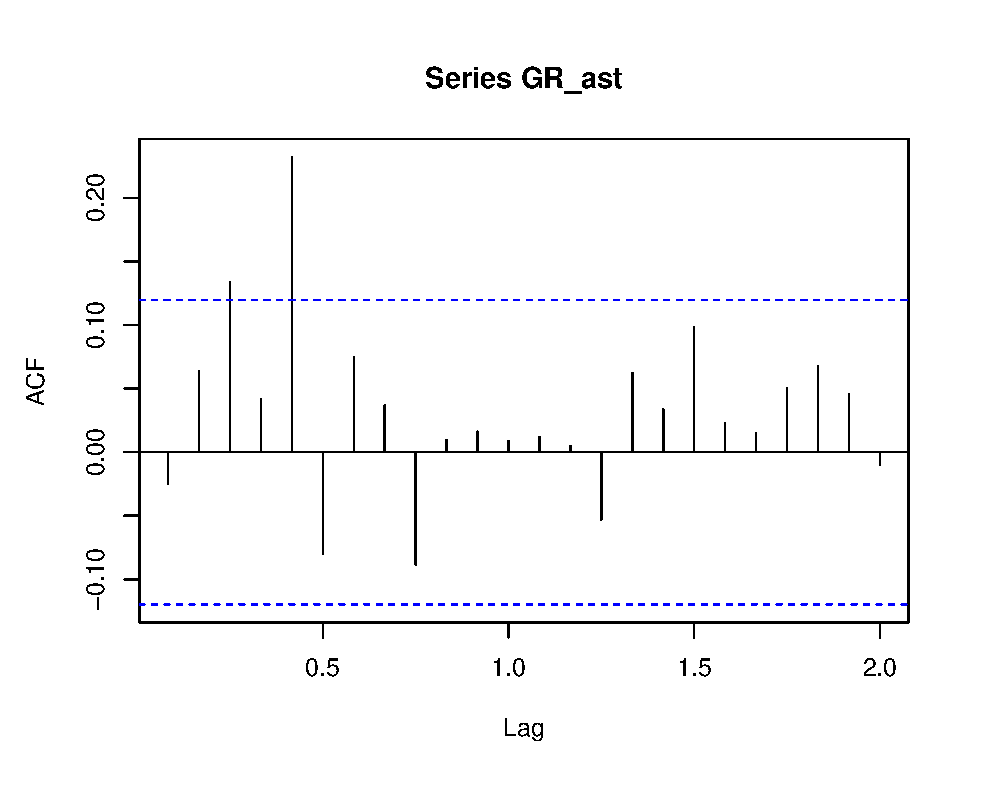
\includegraphics[width=1\textwidth]{pic/acf(gr_ast)}
        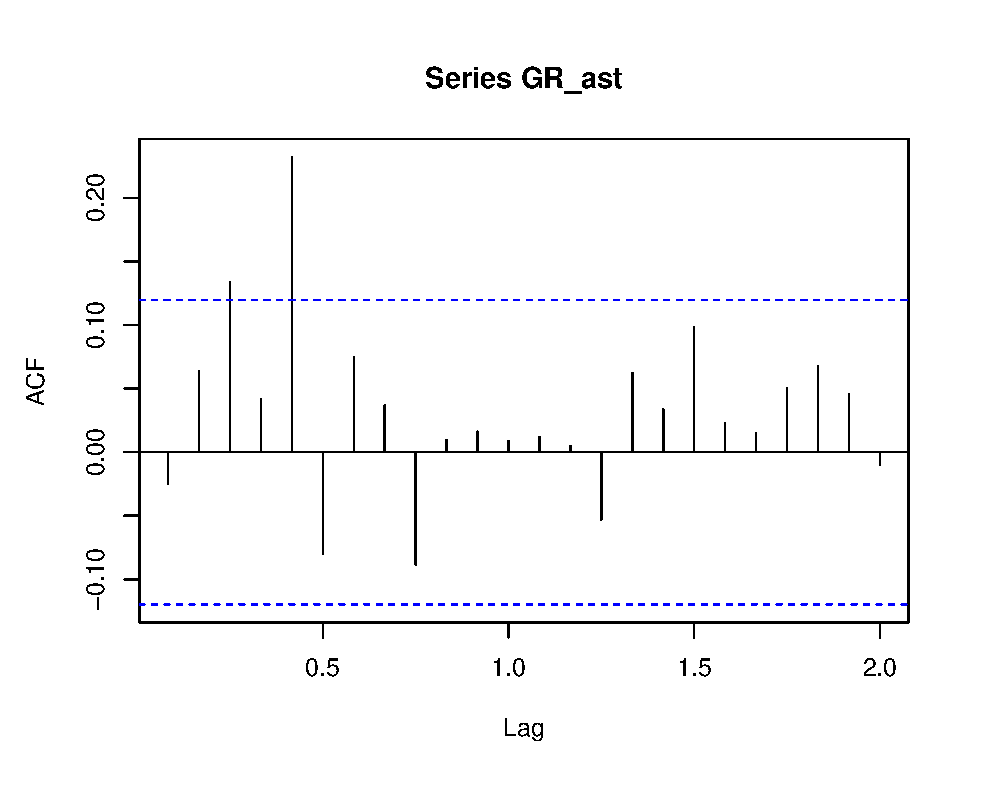
\includegraphics[width=0.5\textwidth]{pic/acf(gr_ast).eps} 
        \subcaption{ACF of GR\_ast}   
        \label{fig:apegrast:a}   
    \end{minipage}
    \begin{minipage}[h]{0.5\textwidth}   
        \centering   
        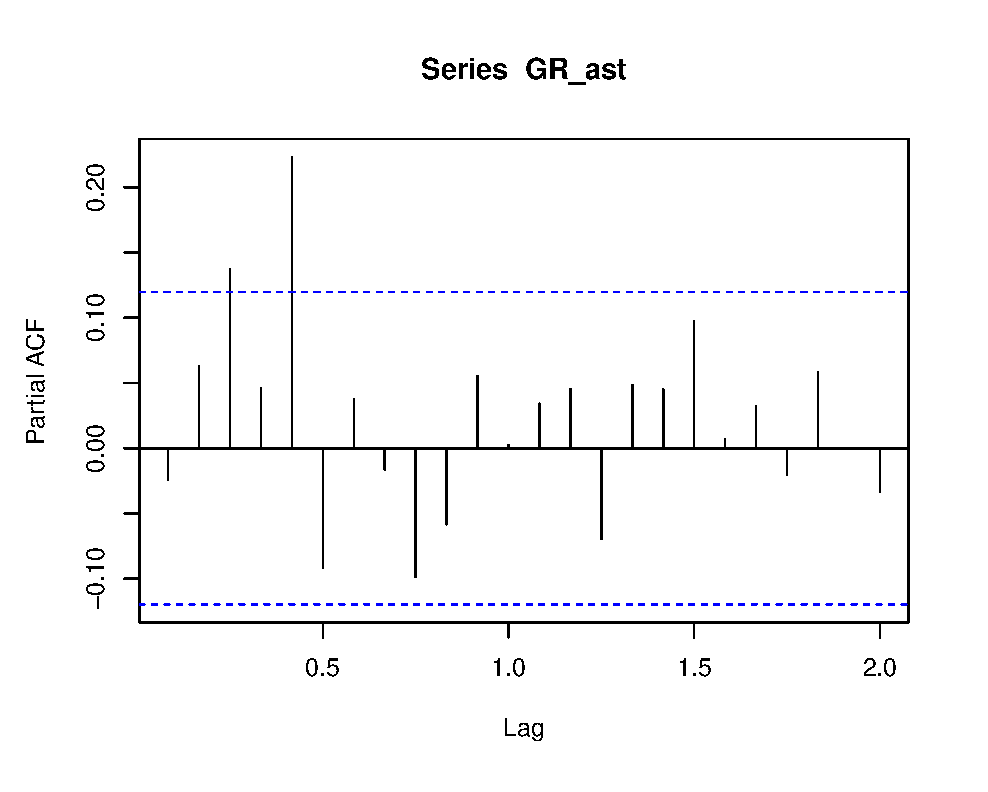
\includegraphics[width=0.5\textwidth]{pic/pacf(gr_ast)}   
        \subcaption{PACF of GR\_ast}   
        \label{fig:pierce:b}   
    \end{minipage}   
    \begin{minipage}[h]{0.5\textwidth} 
        \centering   
        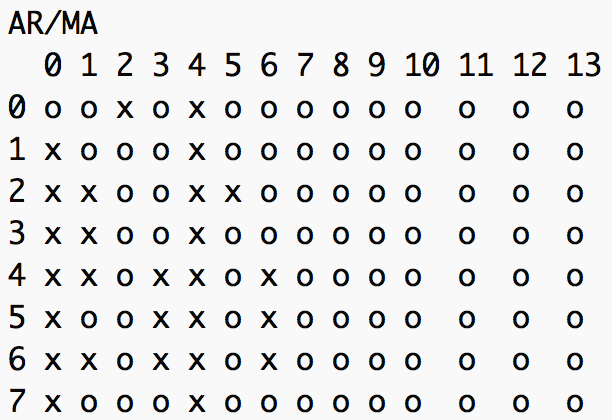
\includegraphics[width=0.5\textwidth]{pic/eacf(gr_ast)}   
        \subcaption{EACF of GR\_ast}   
        \label{fig:apegrast:c}   
    \end{minipage}
    \begin{minipage}[h]{0.5\textwidth} 
    \centering   
    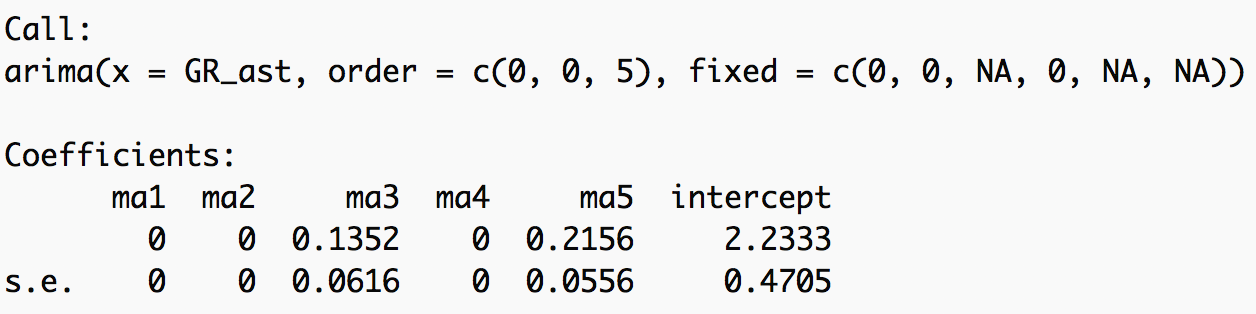
\includegraphics[width=0.5\textwidth]{pic/ma5}   
    \subcaption{MA Model}   
    \label{fig:apegrast:d}   
\end{minipage}    
    \caption{Identify MA Model} 
    \label{fig:apegrast}
\end{multicols}
\end{figure}

\end{document}

